\documentclass[a4paper,10pt]{article}
\usepackage[utf8]{inputenc}

%opening
\title{A Genome Assembly Graph \\
    \smallskip
    \large{DA3018} \\
    \smallskip
    \large{Spring 2019}}
\author{Anton Stråhle \\ 
    Jan Alexandersson \\
    Fredrika Lundahl}

\date{}    

\setlength{\parindent}{0pt}

\newcommand\bref[1]{[\ref{#1}]}

\begin{document}

\maketitle

\section{Introduction}

In this project we examine data consisting of genome assemblies of norwegian spruces. The data set is made up of the starting and ending indexes of the overlap between so called contigs. We let the contigs represent some nodes in a graph whilst the overlap between two contigs creates an edges, which gives us some genome assembly graph which henceforth will be referrd to simply as the graph. 

\medskip

Using this graph we are to find the average degree and the degree distribution. Furthermore we also wish to observe the number of disconnected subgraphs of the genome assembly graph whilst also observing the distribution of the sizes of the subgraphs. 

\medskip

It turns out to be difficult to perform more precise operations on data of this size and as a result we also wish to create some partition method which given the initial graph returns some set of subgraphs containing less than 1000 contigs each. 

\section{Creating the Graph}

In order to create our actual graph we have to translate the actual data set to nodes and edges. In the data set we are given some identifiers for the contigs in question and information regarding their overlap. If an overlap exists between the contigs we create and edge between them. There is however one exception to this rule which is that an edge is not create if one of the contigs is a subsequence of the other. The reason for this is that the occurences of such subsequences is the outcome of containment.

\medskip

Using the set of rules determined in the paragraph above we created a converter which given the input data returns the desired graph. 

\medskip

Running the converter from the data file in order to create the graph worked without problem when using smaller test files but we ran into problems when running it with the whole data set. We got a garbage collection error and after some searching on the Intenet we realised we could just allow Java to use more RAM (Java uses 4G per default) and after giving Java 8G RAM to work with the program ran without error. We reasoned that this is a viable solution as computers nowadays generally have access to at least 8G RAM. 
If we can simply give Java more access to RAM then this solution is the most natural whilst also the being the quickest. So, we run the program using the line "java -Xmx8G DataToGraphConverter ../overlaps.m4", where the flag -Xmx8G specify how much RAM we we give Java access to.

\medskip

When examining the data in order to create our convereter we ovbiosuly could not examine the file as a whole due to its size. To bypass this issue we simply used the unix command ``more'' in order to examine the data page by page. 

\subsection{Graph Representation}

In this project we have choosen to represent our graph using a so called adjacency list. The reasoning behind this is that the useage of an adjacency list holds several advantages compared to representations such as the adjacency matrix. Since the graph will be far from complete we would have a lot of zeros in our matrix which would both occupy more memory and slow down operations on the matrix. By using an adjacency list we avoid these issues and as a result use less memory and get faster operations. It is also preferable to use an adjacency list since it is very easy to derive the degree distribution from it. The only real advantage which an adjacency matrix has over a list is that its far quicker when you want to examine whether or not and edge exists between two nodes. Since this is not something that we have to do in this project it is clear that the adjacency list is far superior to the matrix. 

\section{Degree Distribution Prior to Partitioning}

In order to determine the degree distribution of our graph we simply used the nice functionality of the adjacency list by taking the sizes of each individual list of neighbors. Prior to the partitioning of the graph we were left with the following distribution.

\begin{figure}
	\centering
	\includegraphics[width=\lindwidth]{degreeprior.png}
	\caption{Degree distribution before partitioning}
	\label{fig:degprior}
\end{figure}

As can be seen in Figure \bref{fig:defprior} we have a large number of nodes with degrees of reasonable level, there are however some nodes with degrees that exceed 100 which according to our knowledge should be impossible. When performing our partitions these nodes will be the first to be removed due to            simply being unrealistic.

\section{Distribution of Disconnected Subgraphs Prior to Partitioning}

In order to determine the number of disconnected subgraphs and the sizes of these in our graph we implement a Flood Fill algorithm. The Flood Fill algorithm works by choosing some random node and give it some colour. Then all the neighbors of that node are coloured with the same colour. The procedure is repeated on their neighbors and so on untill there are no nodes left to colour. When this occurs we choose some non-coloured node and give it some different colour. This is repeated until there are no more nodes to colour. The number of different of colours in our graph is the number of disconnected subgraphs whilst the nodes of each colour gives us the size distribution of the subgraphs. In the actual algorithm we let the colours be represented by integers meaning that nodes belong to subgraph $0,1,2,...$. The distribution of the sizes of the subgraphs looks as follows before we partition the graph further.

\begin{figure}
	\centering
	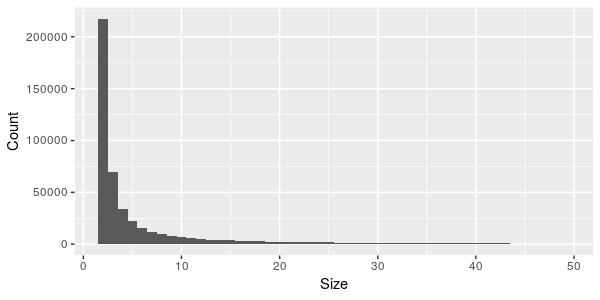
\includegraphics[width=\lindwidth]{sizesprior.png}
	\caption{Size distribution of sungraphs before partitioning}
	\label{fig:sizeprior}
\end{figure}

\section{Partitioning}


\section{Degree Distribution After Partitioning}


\subsection{Distribution of Disconnected Subgraphs After Partitioning}


\section{Time Complexity}



\end{document}




